\documentclass[fleqn]{jbook}
\usepackage{physpub}

\begin{document}

\begin{question}{専攻 問題6}{}


図1は、ロータリー・ポンプP1と油拡散ポンプP2を組み合わせて、測定槽C
を$10^{-4}〜10^{-5}\Unit{Pa}$程度の真空に排気する装置である。
S1,S2はポンプの電源スイッチ、V1〜V5は真空バルブ、Wは給水バルブ、
G1,G2は真空計である。
(注: $1\Unit{Pa} = 1\Unit{N/m^2}=7.5 \Keta{-3} \Unit{Torr}$)


\begin{subquestions}
\SubQuestion
  最初S1,S2はoff,V1からV2およびWは閉の状態にあるとする。
  Cを排気するために行なうべき操作とその目的を、操作の順に番号をつけて
  列挙せよ。なお、途中で20分〜30分待つことが必要であるが、これも操作
  の1項目として扱うこと。また、真空度のチェックも操作の1項目とし、
  どの真空計で何Pa(何Torr)程度になったことをチェックするか、
  真空度のオーダーを記せ。
  (注: 必ずしも決まった順序がない部分は、妥当な順序を一通りだけ示せば
  よい。)

\SubQuestion
  \begin{subsubquestions}
  \SubSubQuestion
    図2(a)はロータリー・ポンプの模式図である。このポンプの動作原理を
    説明する下の文の[ ],( ),$\{ \}$に言葉または記号を入れよ。\\
%
    ただし [ ] には[{\bf 油、吸気口、空気、真空、滑り板、排気口、バネ、弁、偏心、ポンプ}]
    のいずれかの言葉 (解答に使わないものも含まれている)、\\
%
    ( )には図中の部分を示す記号a,b,c,…等 (解答に使わないものも
    含まれている)、\\
%
    $\{ \}$には式を、\\
    \hspace*{1.5cm}例: (1)a,\,(2)b,\,[3] 油,…,$\{18\} V_{1} \times V_{min}$
    のように記せ。

    \vspace*{3mm}

      「固定シリンダー(1)の中心軸にローター(2)が[3]して取り付けられて
    いる。シリンダーには[4](5)がはめられており、[6](7)からの力を受けて
    いる。シリンダー内は、ローターとシリンダーとの接触部(8)、および[4]
    とローターとの接触部によって、2つの空間に分けられている。上部に
    貯められた[9](10)がシリンダー内にしみ出してすべての接触面の隙間を
    埋め、それぞれの空間を気密に保っている。ローターが矢印の向き(時計
    方向)に回転すると、[11]が[12](13)から空間(14)に取り込まれる。一方
    、空間(15)ではすでに取り込まれた[11]が圧縮されつつある。(15)内の
    圧力が1気圧を少し越えると、[16](17)が押し上げられ、[11]は排出される
    。[9]は気密保持と潤滑剤の役割のほかに、重要な役割がある。
    今、空間(14)(15)の体積をそれぞれ$V_{1},V_{2}$とする。$V_{2}$の
    最小値を$V_{min}$とすると、到達真空度はおよそ
    $p_{min}=\{18\}\Unit{Pa}$で与えられると期待される。ところが
    実際のポンプの到達真空度は$p_{min}/1000$に達する。これは[9]が
    体積$V_{min}$を充満するのに十分な量、空間(15)にしみ出しており、
    [11]は[9]中に浮かぶ体積〜$V_{min}/1000$程度の泡にまで圧縮され
    て[9]とともに排出されているからである。」


  \SubSubQuestion
    図2(b)は油拡散ポンプの模式図である。この真空ポンプの動作原理を、
    必要に応じて図中の部分A,B,C,…等の役割に触れながら、6行以内で述
    べよ。また、油拡散ポンプが正常に動作するためには図1のように
    ロータリー・ポンプ等を併用する必要がある。その理由を2行以内で
    述べよ。

  \end{subsubquestions}

\SubQuestion
  \begin{subsubquestions}
  \SubSubQuestion
    数密度$n$の気体中の分子の平均自由行程 $l$ を求めよ。ただし、
    気体分子を直径 $d$ の剛体球と考えてよいものとする。

  \SubSubQuestion
    窒素分子を直径$0.3\Unit{nm}$の剛体球とするとき、温度$300\Unit{K}$
    で、$l=1\Unit{cm}$になるのは圧力$p$が何\Unit{Pa}のときか。
  \end{subsubquestions}
\end{subquestions}
\newpage

\begin{center}
  \mbox{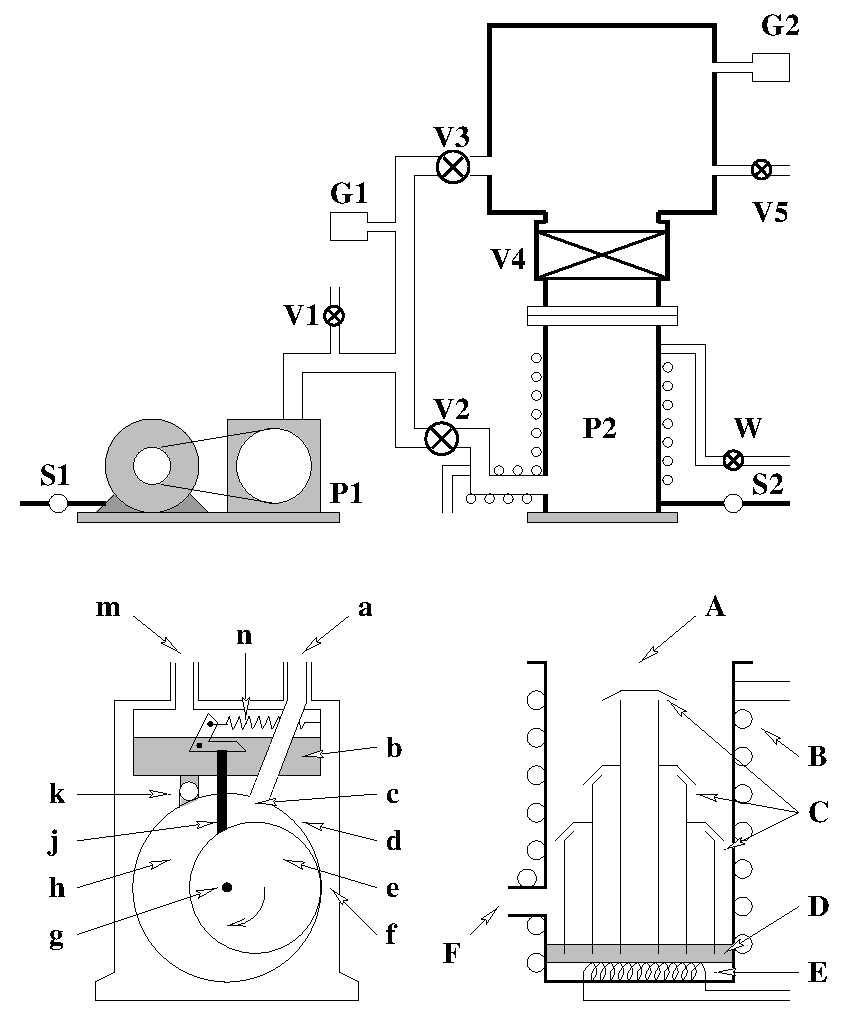
\includegraphics[clip]{1995phy6-1.eps}}
\end{center}

\end{question}
\begin{answer}{専攻 問題6}{}


\begin{subanswers}
\SubAnswer
  やや細かいところもあると思うが、以下のようになるだろう。

  \begin{tabular}{r p{22zw}r p{20zw}}
     & 操作 && 目的 \\
   1 & すべてのバルブが閉じていることと、S1, S2, G1,G2,のスイッチがoffであることを確認する && 真空計の破損や思わぬリークなどを防ぐため \\
   2 & S1をonにする && \\
   3 & P1の音が静かになったらゆっくりV3を開く && P1のポンプ内の空気が引けるのを待つため \\
   4 & 再びP1の音が静かになったらG1をonにする && P2を使用し始めて良いかを確認するため \\
   5 & G1が$6\Unit{Pa}(0.05\Unit{Torr})$ 程度以下になったことをチェックする && (同上) \\
   6 & V3を閉じる && P2内の空気を引くため \\
   7 & V2を開く && (同上) \\
   8 & Wを開く && P2内の油の炭化を防ぐため \\
   9 & S2をonにする && \\
  10 & 20分から30分待つ && P2が暖まるのを待つため \\
  11 & V2を閉じる && P2の準備中にCが$6\Unit{Pa}$ 以上になることがあるが、それを再び $6\Unit{Pa}$ 以下にするため \\
  12 & V3を開く && (同上) \\
  13 & G1が $6\Unit{Pa}(0.05\Unit{Torr})$ 程度以下になったことをチェックする && (同上) \\
  14 & V3を閉じる && (P2のポンプを使用するため) \\
  15 & V2を開く && (同上) \\
  16 & V4を開く && (同上) \\
  17 & ある程度時間が経ったらG2をonにする && \\
  18 & G2が$10^{-4}〜10^{-5}\Unit{Pa}$ 程度であることをチェックする && \\
  \end{tabular}

  注: G2が具体的に与えられていないので、17.でonにする時の条件を
  書かなかったが、G2が、電離真空計(イオンゲージ)なら、C内が
  $0.1\Unit{Pa}(10^{-3}\Unit{Torr})$ 以下になった時にonにすれば良い。
  しかしこの場合でもG1がCに直結していないので、どう確認するかが問題
  になる。




\SubAnswer
  \begin{subsubanswers}
  \SubSubAnswer
    解答は以下の通り\\
    \begin{tabular}{llllllll}
     (1)  & d  & (2)  & e     & [3]  & 偏心 & [4]  & 滑り板 \\
     (5)  & j  & [6]  & バネ  & (7)  & n    & (8)  & f      \\
     $[9]$  & 油 & (10) & b     & [11] & 空気 & [12] & 吸気口 \\
     (13) & a  & (14) & c     & (15) & h    & [16] & 弁     \\
     (17) & k  &$\{18\}$& $V_{\rm min}/(V_1+V_{2}-V_{\rm min})$ &&&& \\
    \end{tabular}

  \SubSubAnswer
    ボイラーEで、油Dを加熱する。発生した油蒸気はノズルCから下向きに
    噴射され、吸気口Aから入ってくる残留ガス分子に下向きの運動量を与
    え、気体を圧縮する。圧縮された気体は、ロータリーポンプ等で排気口
    Fから排気する。また油が蒸気のままでいると油の分子が吸気口に流れて
    ポンプ作用を失い排気速度が落ちる上に、蒸気温度が高くなり過ぎて
    油が分解して使用不可能になる。これを防ぐために水冷パイプBで必ず
    冷却しながら使用する。\\
%
    ロータリーポンプを併用する理由は排気口付近の気体分子の密度が
    大きいと油拡散ポンプ内に逆流し、真空度を上げられないからである。
  \end{subsubanswers}

\SubAnswer
  \begin{subsubanswers}
  \SubSubAnswer
    \parbox[t]{80mm}{
    平均自由行程を概算する方法と Maxwell-Boltzmann分布を用いて
    精密に計算する方法の2通りを示す。\\
%
    まず、概算により平均自由行程を見積もる。\\
%
    数密度$n$の分子が静止していて、その中を同じ分子1個が速さ$u$で
    走る状況を考える。右図はこの状況を走る分子に乗って眺めた図である。
    }\parbox[t]{75mm}{\vspace*{-5mm}
    \begin{center}
      \mbox{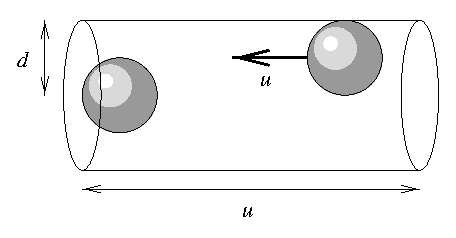
\includegraphics[clip]{1995phy6-2.eps}}
    \end{center}}\\
%
    単位時間にこの分子と衝突する分子はその球の中心が図に示した
    大きさの円柱内部にあるものである。その衝突回数 $N$ は
    $N = \pi d^2 u n$ である。分子の平均衝突時間間隔は $1/N$ で
    与えらるので平均自由行程 $l$ は
%
    \[ l = \frac{1}{N}u = \frac{1}{\pi d^2 n} \]
%
    と得られる。これが概算値である。

    次に Maxwell-Boltzmann分布を用いて平均自由行程を精密に計算する。\\
%
    単位体積中に$n$個ある分子のうち1つの分子に注目した時に、その分子の
    速度が $[\vec{v}_1,\, \vec{v}_1+\d{\vec{v}_1}]$ の範囲にある
    確率は Maxwell-Boltzmann分布 $f(\vec{v})$ を用いて
    $f(\vec{v}_1)\d{\vec{v}_1}$と与えられる。\\
%
    次に他の分子のうち、速度が
    $[\vec{v}_2,\, \vec{v}_2+\d{\vec{v}_2}]$ の範囲にある分子の
    数密度は $n f(\vec{v}_2)\d{\vec{v}_2}$と与えられる。\\
%
    この$\vec{v}_1$の1個の分子と$\vec{v}_2$の多数の分子との衝突のみ
    を考える。$\vec{v}_1$の分子に乗って眺めると、先の図のような
    状況となる。相対速度$u$ は $u=|\vec{v}_1-\vec{v}_2|$ である。
    向かってくる分子の数密度は $n f(\vec{v}_2)\d{\vec{v}_2}$
    であるので、単位時間のこの衝突回数 $N(\vec{v}_1,\vec{v}_2)$ は
%
    \[ N(\vec{v}_1,\vec{v}_2)%
       = \pi d^2 |\vec{v}_1-\vec{v}_2| n f(\vec{v}_2)\d{\vec{v}_2} \]
%
    で与えられる。よってすべての$\vec{v}_1,\vec{v}_2$についての
    $N(\vec{v}_1,\vec{v}_2)$ の和、つまり積分、を求めると、それは
    最初に注目した分子が単位時間に衝突する回数 $N$ となる。
%
    \[ N = \int\!\!\!\int\! \d{\vec{v}_1}\d{\vec{v}_2}%
         \pi d^2 |\vec{v}_1-\vec{v}_2| n f(\vec{v}_1)f(\vec{v}_2) \]
%
    Maxwell-Boltzmann分布 $f(\vec{v})$ の速度依存性は
    $A, \alpha$ を温度などにより決まる定数として
    $f(\vec{v}) = A e^{-\alpha v^2}$と表される。よって、
%
    \[ N=\pi d^2n \int\!\!\!\int\! \d{\vec{v}_1}\d{\vec{v}_2}\,%
         |\vec{v}_1-\vec{v}_2| A^2 e^{-\alpha(v_1^2+v_2^2)} \]
%   
    となる。この積分を計算するために次の変数変換を行う。
%
    \[ \vec{u}_1 = \frac{1}{\sqrt{2}}(\vec{v}_1-\vec{v}_2)%
         \hspace{15mm} %
       \vec{u}_2 = \frac{1}{\sqrt{2}}(\vec{v}_1+\vec{v}_2) \]
%
    \[ \d{\vec{v}_1}\d{\vec{v}_2}%
       = \frac{\partial(\vec{v}_1,\vec{v}_2)}{\partial(\vec{u}_1,\vec{u}_2)}%
         \d{\vec{u}_1}\d{\vec{u}_2}%
       = \d{\vec{u}_1}\d{\vec{u}_2} \hspace{15mm}%
       v_1^2+v_2^2 = u_1^2 + u_2^2 \]
%
    となるのでよって、
%
    \begin{eqnarray*}
     N &=& \sqrt{2}\pi d^2 n%
           \int\!\!\!\int\! \d{\vec{u}_1}\d{\vec{u}_2}\,%
           u_1 A^2 e^{-\alpha(u_1^2+u_2^2)}%
        =  \sqrt{2}\pi d^2 n%
           \int\!\d{\vec{u}_1}\, u_1 A e^{-\alpha u_1^2}%
           \int\!\d{\vec{u}_2}\,     A e^{-\alpha u_2^2} \\
       &=& \sqrt{2}\pi d^2 n%
           \int\!\d{\vec{v}}\, v f(\vec{v})%
           \int\!\d{\vec{v}}\,   f(\vec{v})%
        =  \sqrt{2}\pi d^2 n \cdot \Mean{v} \cdot 1
    \end{eqnarray*}
%
    よって平均自由行程 $l$ は
%
    \[ l = \frac{1}{N} \Mean{v} = \frac{1}{\sqrt{2}\pi d^2 n} \]
%
    と得られる。これが精密値である。

  \SubSubAnswer
    $p=nk_B T$より
%
    \[ p  = \frac{1}{\sqrt{2}l\pi d^2} k_B T %
          = \frac{1.38\Keta{-23} \Unit{J/K} \cdot 300 \Unit{K}}{\sqrt{2}\cdot 1\Keta{-2}\Unit{m}\times \pi \cdot (0.3\Keta{-9}\Unit{m})^2}%
          = 1.04 \Unit{Pa} \]
%
  \end{subsubanswers}
\end{subanswers}
\end{answer}



\end{document}
